\begin{figure}[t]
%\captionsetup[subfigure]{justification=centering}
\begin{subfigure}[t]{0.48\textwidth}
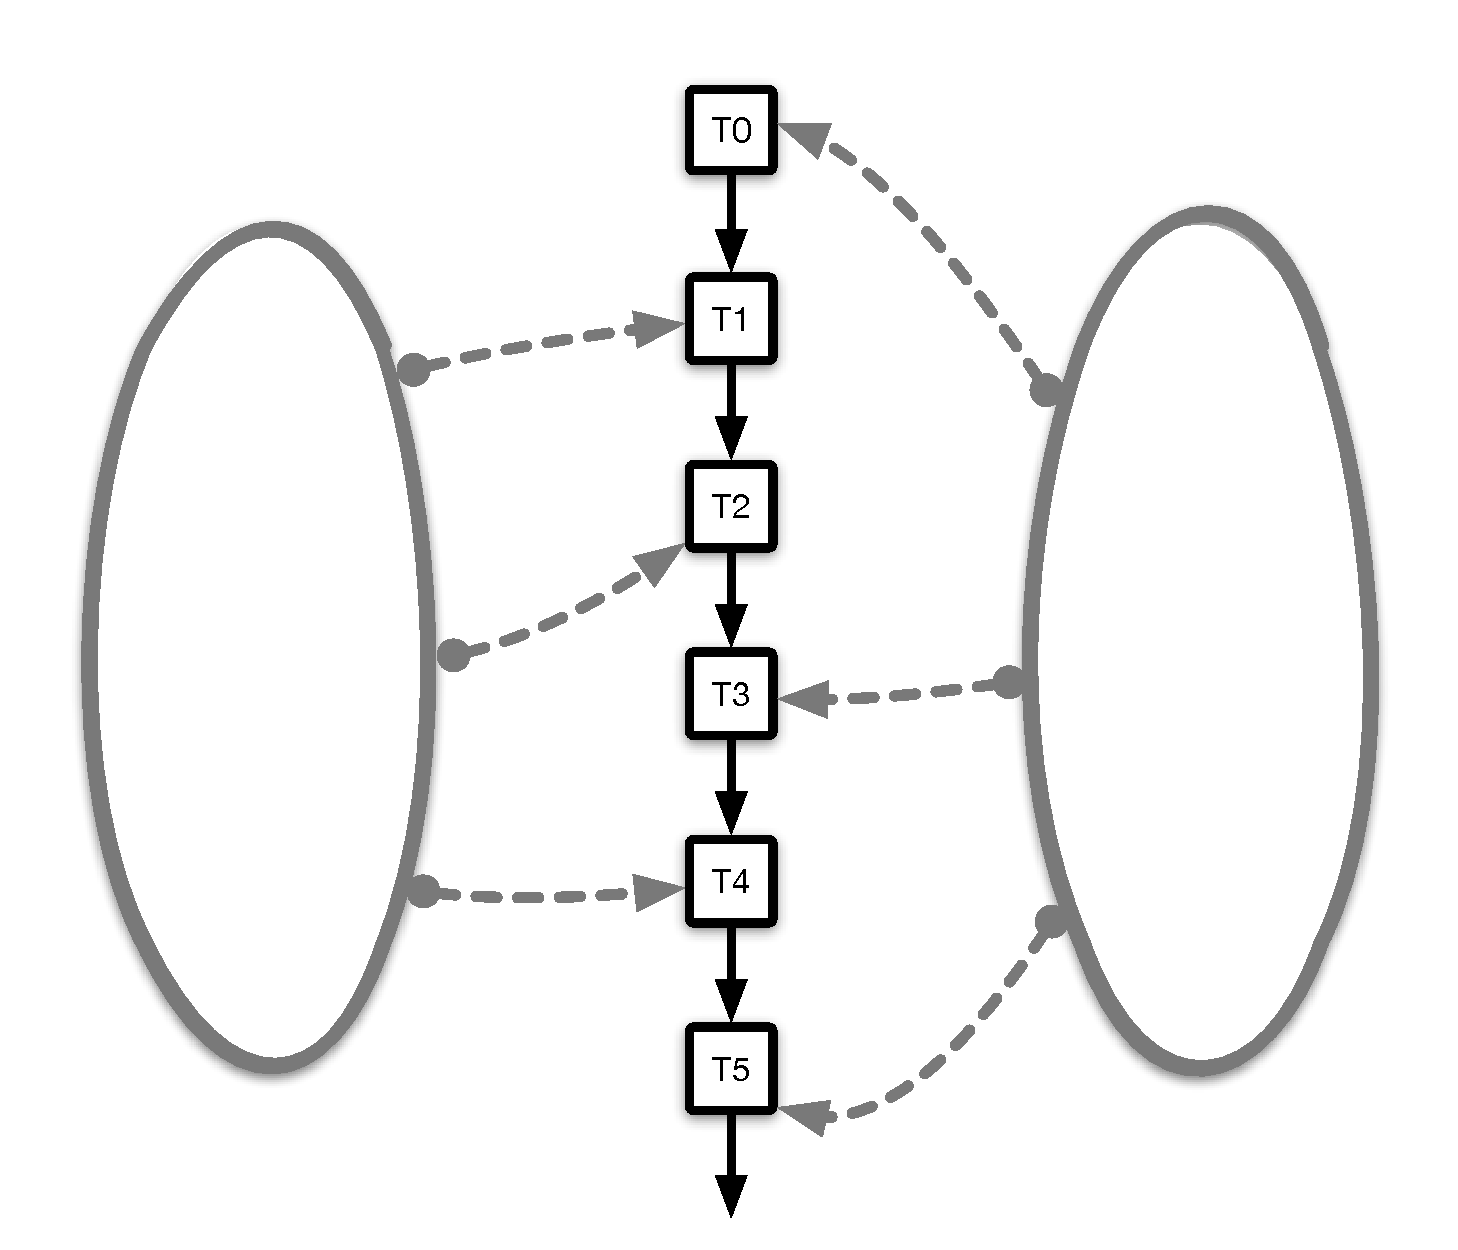
\includegraphics[height=4cm]{res/before-cloud.pdf}
\caption{\label{fig:relink:intro:before}}
\end{subfigure} \hfill
\begin{subfigure}[t]{0.48\textwidth}
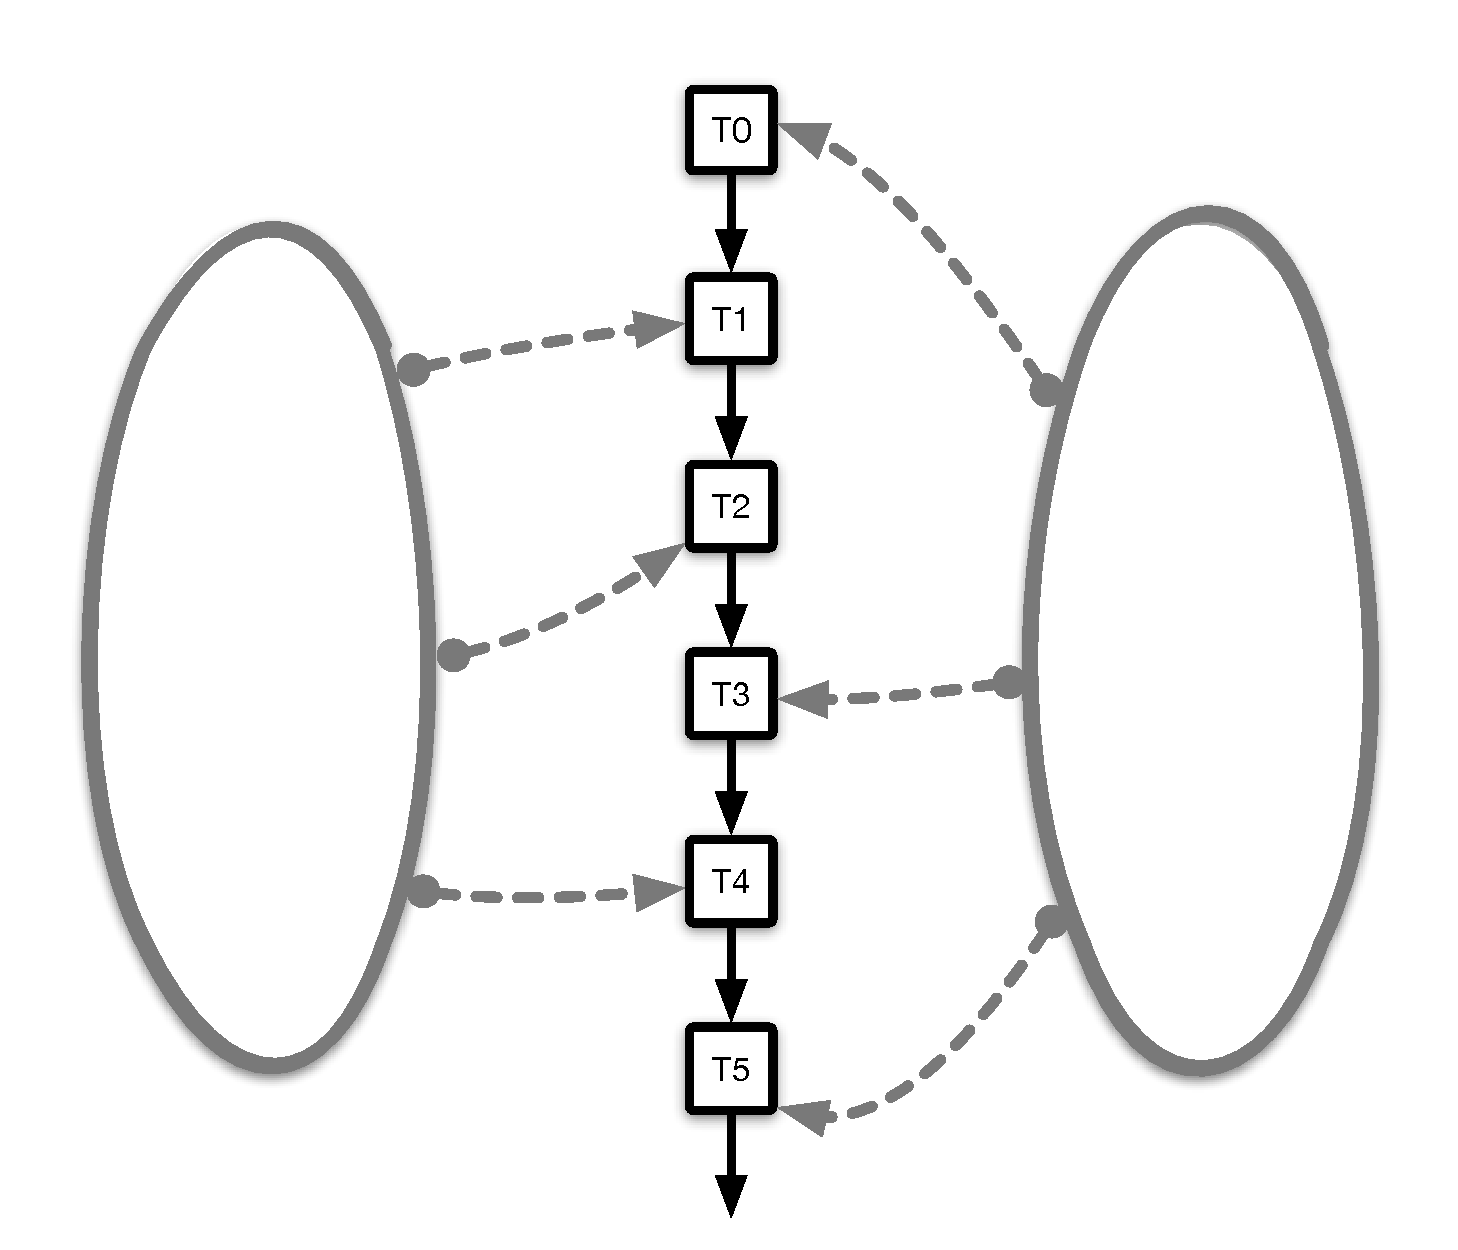
\includegraphics[height=4cm]{res/before-cloud.pdf}
\caption{\label{fig:relink:intro:after}} % Logical $\neq$ Real Time order, snapshot OK}
\end{subfigure}%
%
\caption{\label{fig:relink:intro} Placeholder for a general
  picture. The list ordering the events $T_0-T_5$ is permutted from
  (a) to (b), while preserving the event ownership: $T_1$, $T_2$ and
  $T_4$ have been executed---and are thus owned---by the specified
  thread (aka.~self), while $T_0$, $T_3$ and $T_5$ are executed by the
  interfering threads (aka.~other).}
\end{figure}
